\chapter{Navier-Stokes Equations - Part 1}
\label{ch:nsderive1}

\section{Learning objectives}

At the end of this lesson, a student should be able to
\begin{enumerate}
\item perform algebraic analysis using subscript notation
\item identify the terms and their role in the Navier-Stokes equations
\item recall Navier-Stokes equations in rectangular coordinate system
\item derive and recall definition of Reynold's number
\item analyse the dominant terms of Navier-Stokes equations for small and large values of Reynold's number
\end{enumerate}

\section{Concept map}

% learning objective
\begin{lo2}[Fluid Flow]
  List the concepts behind Navier-Stokes equations
\end{lo2}

The starting point for momentum balance equation is Newton's second law of motion applied to a moving volume element in a fluid.


The strategy to derive Navier-Stokes equation \index{Navier-Stokes equation} is illustrated in the concept map below.

\begin{figure}[h]
 \centering
 \includegraphics[width=6 in]{images/c09-NavierStokesFlowChart2.eps}
 % ctrans.eps: 46x0 pixel, 300dpi, 0.39x0.00 cm, bb=0 35 595 420
 \caption{Concept map of derivation of Navier-Stokes equation}
 \label{nsconceptmap}
\end{figure}


\section{Forces}

{\bf Long range forces} decrease slowly with increase in distance between the interacting elements. These are called body forces or volume forces. Examples such as gravity (due to density $\rho$ gradients), electromagnetic (in metals carrying electric currents) and fictitious (centrifugal or coriolis) act on the whole of the fluid element and are usually proportional to the size of the volume element ($\delta V$). They can be represented as:

$$ F_i(x_i,t) \rho \delta V $$

Eg. gravity pointing vertically downwards :

$$ F_i = g \hat{x}_2 $$

{\bf Short range forces} decrease rapidly with increase in distance between the interacting elements and are of molecular origin. Examples such as forces applied on surfaces (normal and shear), Marangoni forces (due to surface tension gradients) act on a thin layer of the fluid and are called surface forces. Local short range forces exerted by the fluid on different surface elements ($\delta A$) can be represented as:

$$ \sigma(x_i, n_j, t) \delta A $$

where, $n_j$ is the unit normal to the surface element $\delta A$. $\sigma$ is called the local {\bf stress}.

\section{Equation of motion}

% learning objective
\begin {lo3} [Fluid Flow]
Derive equation of motion
\end {lo3}

Consider a moving fluid element of volume $dV$ and area $dS$ on a surface with normal $n_i$. Using the material derivative $\frac{D}{Dt}$ introduced earlier, the rate of change of momentum of a small fluid element of volume $dv$ is given by:

$$ \frac{D}{Dt} \int_{V}{\rho u_i dV} $$

Using the Reynold's transport theorem \index{Reynolds transport theorem} [\ref{rtt}] and the continuity equation, one can bring the material derivative inside the integral as illustrated in section [\ref{ktt}]. 

$$ \frac{D}{Dt} \int_{V}{\rho u_i dV} =  \int_{V}{\rho \frac{Du_i}{Dt} dV} $$

The total force that acts on $dV$ is the sum of body forces and surface forces:

$$ \int_{V}{F_i\rho dV} + \int_{S}{\sigma_{ij}n_jdS} $$

Using Gauss divergence theorem, \index{Gauss Divergence theorem}

\begin{equation}
\int_{S}{\sigma_{ij}n_jdS} = \int_{V}{\frac{\partial \sigma_{ij}}{\partial x_j}dV}
\end{equation} 

From Newton's second law, the rate of change of momentum is equal to the total force acting on the element. Hence,

\begin{equation}
\int_{V}{\frac{Du_i}{Dt}\rho dV}  =  \int_{V}{F_i\rho dV} + \int_{V}{\frac{\partial \sigma_{ij}}{\partial x_j}dV}
\end{equation} 

Since the three integrands are being summed over the same volume element, it will be applicable at {\em any} location in the fluid if the equation applies to the integrands themselves:

\begin{equation}
\label{eqmotion}
\boxed{\frac{Du_i}{Dt}\rho =  F_i\rho + \frac{\partial \sigma_{ij}}{\partial x_j}}
\end{equation} 

We now need to express $\sigma_{ij}$ in a way that can minimise the number of unknown parameters in the above equation of motion.

\section{Stress tensor}

Section \ref{cauchy} stating the Cauchy's stress principle and section \ref{stresstensor} prove that stress is a tensor. We can also use conservation of angular momentum to show that the stress tensor is symmetric as described in section \ref{symstress}. Hence it can be expressed as 

\begin{equation}
\sigma_{ij} = \left(
\begin{array}{lll}
\sigma_{11} & \sigma_{12} & \sigma_{13} \\ 
\sigma_{12} & \sigma_{22} & \sigma_{23} \\ 
\sigma_{13} & \sigma_{23} & \sigma_{33} \\ 
\end{array}
\right)
\end{equation} 

Since it is always possible to find a co-ordinate system such that the matrix containing the elements of a symmetric tensor is diagonal, we can write $\sigma_{ij}$ as the follows.


\begin{equation}
\sigma_{ij} = \left(
\begin{array}{lll}
\sigma_{11} & 0 & 0 \\ 
0 & \sigma_{22} & 0 \\ 
0 & 0 & \sigma_{33} \\ 
\end{array}
\right)
\end{equation} 

or 

\begin{equation}
\sigma_{ij} = \left(
\begin{array}{lll}
\frac{1}{3}\sigma_{kk} & 0 & 0 \\ 
0 & \frac{1}{3}\sigma_{kk} & 0 \\ 
0 & 0 & \frac{1}{3}\sigma_{kk} \\ 
\end{array}
\right) + \left(
\begin{array}{lll}
\sigma_{11}-\frac{1}{3}\sigma_{kk} & 0 & 0 \\ 
0 & \sigma_{22}-\frac{1}{3}\sigma_{kk} & 0 \\ 
0 & 0 & \sigma_{33}-\frac{1}{3}\sigma_{kk} \\ 
\end{array}
\right) 
\end{equation} 

where

\begin{equation}
\sigma_{kk}=\sigma_{11} + \sigma_{22} + \sigma_{33}
\end{equation} 

\begin{equation}
\sigma_{ij} = \frac{1}{3}\sigma_{kk}\delta_{ij} +  d_{ij}
\end{equation} 

We define static pressure of the fluid with the convention that positive pressure is that which acts to compress a fluid element,

\begin{equation}
p = -\frac{1}{3}\sigma_{kk}
\end{equation} 

so that 

\begin{equation}
\label{sigmaij}
\sigma_{ij} = -p\delta_{ij} +  d_{ij}
\end{equation} 

\index{Deviatoric stress}
$d_{ij}$ is called the {\em deviatoric} part of the tensor and leads only to volume conserving deformation of the fluid elements ie., flow of the fluid. Static pressure, on the other hand, leads to a shape-conserving change in the volume element. It is easy to note that 

\begin{equation}
d_{kk} = 0
\end{equation} 

We have separated the stress into two terms:
\begin{itemize}
\item 
{\em pressure} \index{Pressure} term ($-p\delta_{ij}$) that tends to change the volume of a fluid element 
\item 
{\em deviatoric stress} term ($d_{ij}$) that tends to change the shape of a fluid element while keeping the volume constant
\end{itemize}

By analysing all modes of change of shape of a fluid element, we can relate the deviatoric stress with the terms that quantify the shape changes of a fluid element. For non-zero velocity field, because the fluid element translates as time progresses, we will notice that rate of change of shape is more appropriate to analyse a fluid element.

\section{Strain rate tensor}

\index{Strain rate tensor}

The meaning of velocity gradient or a strain rate term $\frac{\partial u_i}{\partial x_j}$ is given in section \ref{strainratemeaning}. Proof that velocity gradient is a tensor of order two is given in section \ref{strainratetensor}. Strain rate or velocity gradient is represented as below and can be shown to be a second order tensor and thus expressible as a sum of symmetric and anti-symmetric tensors. 

\begin{equation}
\frac{\partial u_i}{\partial x_j} = e_{ij} + \Omega_{ij} 
\end{equation} 

\begin{equation}
e_{ij} = \frac{1}{2} \left( \frac{\partial u_i}{\partial x_j} + \frac{\partial u_j}{\partial x_i} \right) 
\end{equation} 

\begin{equation}
\Omega_{ij} = \frac{1}{2} \left( \frac{\partial u_i}{\partial x_j} - \frac{\partial u_j}{\partial x_i} \right) 
\end{equation} 

Define $\omega$ as 

\begin{equation}
\vec{\omega} = \vnabla \times \vec{u} 
\end{equation} 

or

\begin{equation}
\omega_i = \epsilon_{ijk}u_{j,k} = \epsilon_{ijk} \frac{\partial u_j}{\partial x_k} 
\end{equation} 

so that,

\begin{equation}
\Omega_{ij} = -\frac{1}{2}\epsilon_{ijk}\omega_k
\end{equation} 


\section{Relation between stress and strain-rate}

A relation between the deviatoric stress and strain-rate (velocity gradient) is necessary to proceed further to be able to use the equation of motion to solve for the velocity $u_i$. We have to adopt a {\em phenomenological} approach. 

\begin{list}{}{}
\item By definition, $d_{ij}$ is the deviatoric stress which implies that it is zero for a stationary fluid.
\item The velocities and thus the velocity gradients $\frac{\partial u_i}{\partial x_j}$ are zero for a stationary fluid.
\item The deviatoric stress represents the frictional interaction between different layers of the fluid and is assumed to be dependent only on the instantaneous and local distribution of the velocities. 
\end{list} 

From the above observations, we may {\em assume} that the deviatoric stress and the strain-rate are directly and {\em linearly} related to each other. Since both the quantities are tensors of order two, the entity that connects them both must be a tensor of order four.

\begin{equation}
d_{ij} = A_{ijkl} \frac{\partial u_k}{\partial x_l}
\end{equation} 

Since the above equation connects an effect with a cause, it is a {\em constitutive relation}
and the entity $A_{ijkl}$ is a physical parameter. The material in concern is a fluid in which a directionality can safely be assumed to be absent ie., 

\begin{center}
{\em fluids are isotropic}
\end{center}

 Hence, $A_{ijkl}$ must possess the same properties as that of an isotropic tensor of order four. From the properties of tensors, we know that the general form of an isotropic tensor of order four [\ref{isotensorfour}] is 

\begin{equation}
A_{ijkl} = \mu_1 \delta_{ij}\delta_{kl} + \mu_2 \delta_{il}\delta_{kj} + \mu_3 \delta_{ik}\delta_{jl}
\end{equation} 

Since deviatoric stress $d_{ij}$ is symmetric, interchanging the subscripts $i$ and $j$ should keep the quantity identical. In the above equation, this applies also to the R.H.S. ie.,

\begin{equation}
A_{ijkl} = A_{jikl} \Rightarrow \mu_2 = \mu_3
\end{equation} 

\begin{equation}
A_{ijkl} = \mu_1 \delta_{ij}\delta_{kl} + \mu_2 \left( \delta_{il}\delta_{kj} + \delta_{ik}\delta_{jl} \right)
\end{equation} 

$A_{ijkl}$ is now symmetrical in $k$ and $l$ also.

Expanding the above equation,

\begin{equation}
d_{ij} = A_{ijkl} \left( e_{kl} + \Omega_{kl} \right)
\end{equation} 

Since $A_{ijkl}$ is now symmetrical in $k$ and $l$, when it is multiplied by an entity that is anti-symmetric about $k$ and $l$ and the terms are summed over $k$ and $l$ they vanish. Thus, the $\Omega_{kl}$ term drops out.

\begin{equation}
d_{ij} = \left( \mu_1 \delta_{ij}\delta_{kl} + \mu_2 \left( \delta_{il}\delta_{kj} + \delta_{ik}\delta_{jl} \right) \right) e_{kl}
\end{equation} 

\begin{equation}
d_{ij} = \mu_1 \delta_{ij}\delta_{kl}e_{kl} + \mu_2 \left( \delta_{il}\delta_{kj}e_{kl} + \delta_{ik}\delta_{jl}e_{kl} \right)
\end{equation} 

\index{Compressibility}
\index{Rate of dilation}
\index{Rate of expansion}

We have already (\ref{rdiln}) defined {\em compressibility} or {rate of dilation} or rate of expansion as

\begin{equation}
e_{kk} = \frac{\partial u_1}{\partial x_1} + \frac{\partial u_2}{\partial x_2} + \frac{\partial u_3}{\partial x_3} = \Delta 
\end{equation} 

For the first term, we use the contraction theorem [section \ref{contraction}] to get

\begin{equation}
d_{ij} = \mu_1 \delta_{ij}\Delta + 2 \mu_2 e_{ij}
\end{equation} 

Recalling that $d_{ii}=0$,

\begin{equation}
d_{ii} = \mu_1 3 \Delta + 2 \mu_2 \Delta = (3 \mu_1 + 2 \mu_2) \Delta = 0
\end{equation} 

We would like the above equation to be true also for incompressible fluids ie., also when $\Delta \ne 0$. It can be true only when the term in parantheses vanishes.

\index{Stokes assumption}

{\em Stokes' Assumption}: For monoatomic fluids since there is no conversion of translational energy into vibrationary / rotationary energies, {\em bulk viscosity} can be assumed to be zero:

$$(3 \mu_1 + 2 \mu_2)=0$$ 

or

\begin{equation}
\mu_1 = -\frac{2}{3} \mu_2 
\end{equation} 

Watch out for fluids for which Stokes' assumption is not valid. 

Calling the one constant parameter as $\mu$, the equation becomes

\begin{equation}
d_{ij} = - \frac{2}{3} \mu \delta_{ij} \Delta + 2 \mu e_{ij}
\end{equation} 

\begin{equation}
\label{dij}
d_{ij} = 2 \mu \left( e_{ij} - \frac{1}{3} \Delta \delta_{ij} \right)
\end{equation} 


Now that we have an expression for $d_{ij}$ in terms of velocity gradients, we can substitute the same in the equation of motion.

\section{Navier-Stokes equations}

\index{Navier-Stokes equation}

Combining equation of motion (\ref{eqmotion}) and the expressions for stress tensor (\ref{sigmaij} and \ref{dij}), we get,

\begin{equation}
\rho \frac{Du_i}{Dt} = \rho F_i + \frac{\partial}{\partial x_j} \left[ -p\delta_{ij}+ 2 \mu \left( e_{ij} - \frac{1}{3} \Delta \delta_{ij}\right)\right]
\end{equation} 

Expanding the term $e_{ij}$ and using the kronecker delta to contract subscripts, we get:

\begin{equation}
\rho \frac{Du_i}{Dt} = \rho F_i -  \frac{\partial p}{\partial x_i} +  
\frac{\partial}{\partial x_j} \left( \mu \frac{\partial u_i}{\partial x_j} \right) + 
\frac{\partial}{\partial x_j} \left( \mu \frac{\partial u_j}{\partial x_i} \right) + 
\frac{\partial}{\partial x_i} \left( -\frac{2}{3} \mu \Delta \right) 
\end{equation} 

Since the order of differentiation should not matter and if $\mu$ is not a function of location,
\begin{equation}
\rho \frac{Du_i}{Dt} = \rho F_i -  \frac{\partial p}{\partial x_i} +  
\frac{\partial}{\partial x_j} \left( \mu \frac{\partial u_i}{\partial x_j} \right) + 
\frac{\partial}{\partial x_i} \left( \mu \frac{\partial u_j}{\partial x_j} \right) + 
\frac{\partial}{\partial x_i} \left( -\frac{2}{3} \mu \Delta \right) 
\end{equation} 

\begin{equation}
\rho \frac{Du_i}{Dt} = \rho F_i -  \frac{\partial p}{\partial x_i} +  
\frac{\partial}{\partial x_j} \left( \mu \frac{\partial u_i}{\partial x_j} \right) + 
\frac{\partial}{\partial x_i} \left( \mu \Delta \right) + 
\frac{\partial}{\partial x_i} \left( -\frac{2}{3} \mu \Delta \right) 
\end{equation} 


\begin{equation}
\label{ns0}
\boxed{
\rho \frac{Du_i}{Dt} = \rho F_i -  \frac{\partial p}{\partial x_i} +  
\frac{\partial}{\partial x_j} \left( \mu \frac{\partial u_i}{\partial x_j} \right) + 
\frac{1}{3}\frac{\partial}{\partial x_i} \left( \mu \Delta \right) 
}
\end{equation} 

The above set of three equations (for $i=1,2,3$) corresponding to the three components of the velocity of the fluid ($u_1$, $u_2$ and $u_3$) is called {\bf Navier-Stokes equations}.

% which are also given below in expanded form for cartesian co-ordinate system:

%\begin{align}
%\label{ns1}
%\rho \left[ 
%\frac{\partial u_1}{\partial t} + u_1\frac{\partial u_1}{\partial x_1} + u_2\frac{\partial u_1}{\partial x_2} + u_3\frac{\partial %u_1}{\partial x_3} 
%\right] & = \rho F_1 -  \frac{\partial p}{\partial x_1} \nonumber \\
%& + \frac{\partial}{\partial x_1} \left(\mu \frac{\partial u_1}{\partial x_1}\right) + \frac{\partial}{\partial x_2} \left( \mu %\frac{\partial u_1}{\partial x_2} \right) + \frac{\partial}{\partial x_3} \left( \mu \frac{\partial u_1}{\partial x_3} \right) \nonumber \\
%& + \frac{1}{3} \frac{\partial}{\partial x_1} \left[ \mu \left( \frac{\partial u_1}{\partial x_1} + \frac{\partial u_2}{\partial x_2} + %\frac{\partial u_3}{\partial x_3} \right)\right]
%\end{align} 

%\begin{align}
%\label{ns2}
%\rho \left[ 
%\frac{\partial u_2}{\partial t} + u_1\frac{\partial u_2}{\partial x_1} + u_2\frac{\partial u_2}{\partial x_2} + u_3\frac{\partial %u_2}{\partial x_3} 
%\right] & = \rho F_2 -  \frac{\partial p}{\partial x_2} \nonumber \\
%& + \frac{\partial}{\partial x_1} \left(\mu \frac{\partial u_2}{\partial x_1}\right) + \frac{\partial}{\partial x_2} \left( \mu %\frac{\partial u_2}{\partial x_2} \right) + \frac{\partial}{\partial x_3} \left( \mu \frac{\partial u_2}{\partial x_3} \right) \nonumber \\
%& + \frac{1}{3} \frac{\partial}{\partial x_2} \left[ \mu \left( \frac{\partial u_1}{\partial x_1} + \frac{\partial u_2}{\partial x_2} + %\frac{\partial u_3}{\partial x_3} \right)\right]
%\end{align} 

%\begin{align}
%\label{ns3}
%\rho \left[ 
%\frac{\partial u_3}{\partial t} + u_1\frac{\partial u_3}{\partial x_1} + u_2\frac{\partial u_3}{\partial x_2} + u_3\frac{\partial %u_3}{\partial x_3} 
%\right] & = \rho F_3 -  \frac{\partial p}{\partial x_3} \nonumber \\
%& + \frac{\partial}{\partial x_1} \left(\mu \frac{\partial u_3}{\partial x_1}\right) + \frac{\partial}{\partial x_2} \left( \mu %\frac{\partial u_3}{\partial x_2} \right) + \frac{\partial}{\partial x_3} \left( \mu \frac{\partial u_3}{\partial x_3} \right) \nonumber \\
%& + \frac{1}{3} \frac{\partial}{\partial x_3} \left[ \mu \left( \frac{\partial u_1}{\partial x_1} + \frac{\partial u_2}{\partial x_2} + %\frac{\partial u_3}{\partial x_3} \right)\right]
%\end{align} 

%Equations \ref{ns1}, \ref{ns2} and \ref{ns3} are the Navier-Stokes equations in cartesian co-ordinate system in complete form applicable for both compressible as well as incompressible Newtonian fluids. 

If the fluid being considered is incompressible, we can set the last term to zero and obtain the N-S equation with variable property.

A further simplification can be done starting from equation \ref{ns0} as follows. Most of the fluids under normal flow conditions are {\em incompressible} ie., $\Delta=0$. The Navier-Stokes equations for {\em incompressible} fluid flow with {\em constant viscosity} are obtained by taking $\mu$ out of the derivative and setting $\Delta=0$ in the equation~\ref{ns0}.

\begin{equation*}
\rho \frac{Du_i}{Dt} = \rho F_i -  \frac{\partial p}{\partial x_i} +  
\mu \frac{\partial^2 u_i}{\partial x_j^2} + \mu \left(\frac{\partial^2 u_j}{\partial x_j \partial x_i} \right) 
\end{equation*} 

\begin{equation*}
\rho \frac{Du_i}{Dt} = \rho F_i -  \frac{\partial p}{\partial x_i} +  
\mu \frac{\partial^2 u_i}{\partial x_j^2} + \mu \frac{\partial}{\partial x_i} \left(\frac{\partial u_j}{\partial x_j} \right) 
\end{equation*} 

\begin{equation*}
\rho \frac{Du_i}{Dt} = \rho F_i -  \frac{\partial p}{\partial x_i} +  
\mu \frac{\partial^2 u_i}{\partial x_j^2} + \mu \frac{\partial}{\partial x_i} \left(\Delta \right) 
\end{equation*} 

\begin{equation}
\label{nsa}
\rho \frac{Du_i}{Dt} = \rho F_i -  \frac{\partial p}{\partial x_i} +  
\mu \frac{\partial^2 u_i}{\partial x_j^2} 
\end{equation} 

Expanding the material derivative $\frac{D}{Dt}$ and writing in vector notation:

\begin{eqnarray}
\label{nsan}
\frac{\partial u_1}{\partial t} + (\vec{u}\cdot\vnabla)u_1 = F_1 -  \frac{1}{\rho} \frac{\partial p}{\partial x_1} +  \frac{\mu}{\rho} \nabla^2 u_1 
\nonumber \\
\frac{\partial u_2}{\partial t} + (\vec{u}\cdot\vnabla)u_2 = F_2 -  \frac{1}{\rho} \frac{\partial p}{\partial x_2} +  \frac{\mu}{\rho} \nabla^2 u_2 
\nonumber \\
\frac{\partial u_3}{\partial t} + (\vec{u}\cdot\vnabla)u_3 = F_3 -  \frac{1}{\rho} \frac{\partial p}{\partial x_3} +  \frac{\mu}{\rho} \nabla^2 u_3 
\end{eqnarray} 

These can be expanded to give the N-S equations for incompressible fluids of constant property using the definition of kinematic viscosity as follows:
$$\nu = \frac{\mu}{\rho}$$

\begin{equation}
\label{nsa1}
\boxed{
\frac{\partial u_1}{\partial t} + u_1\frac{\partial u_1}{\partial x_1} + u_2\frac{\partial u_1}{\partial x_2} + u_3\frac{\partial u_1}{\partial x_3} = F_1 -  \frac{1}{\rho}\frac{\partial p}{\partial x_1} + \nu \left( \frac{\partial^2 u_1}{\partial x_1^2} + \frac{\partial^2 u_1}{\partial x_2^2} + \frac{\partial^2 u_1}{\partial x_3^2} \right)
}
\end{equation} 

\begin{equation}
\label{nsa2}
\boxed{
\frac{\partial u_2}{\partial t} + u_1\frac{\partial u_2}{\partial x_1} + u_2\frac{\partial u_2}{\partial x_2} + u_3\frac{\partial u_2}{\partial x_3} = F_2 -  \frac{1}{\rho}\frac{\partial p}{\partial x_2} + \nu \left( \frac{\partial^2 u_2}{\partial x_1^2} + \frac{\partial^2 u_2}{\partial x_2^2} + \frac{\partial^2 u_2}{\partial x_3^2} \right)
}
\end{equation} 

\begin{equation}
\label{nsa3}
\boxed{
\frac{\partial u_3}{\partial t} + u_1\frac{\partial u_3}{\partial x_1} + u_2\frac{\partial u_3}{\partial x_2} + u_3\frac{\partial u_3}{\partial x_3} = F_3 -  \frac{1}{\rho}\frac{\partial p}{\partial x_3} + \nu \left( \frac{\partial^2 u_3}{\partial x_1^2} + \frac{\partial^2 u_3}{\partial x_2^2} + \frac{\partial^2 u_3}{\partial x_3^2} \right)
}
\end{equation} 

The continuity equation \ref{conteq2} and the three N-S equations \ref{ns0} are solved together to obtain fluid flow. In these four equations, we have four variables $(p, u_1, u_2, u_3)$ - thus the problem is well defined.

% --------- end of momentum.tex ---------------------------------
